\section[Operations Research Model]{Operations Research Model}
\subsection[Steel Production Data Analysis]{Steel Production Data Analysis}
%\subsubsection[Association Networks]{Association Networks}
\begin{frame}
	\frametitle{Association Networks}
	\begin{columns}[c]
		\column{.5\textwidth}
		\centering
		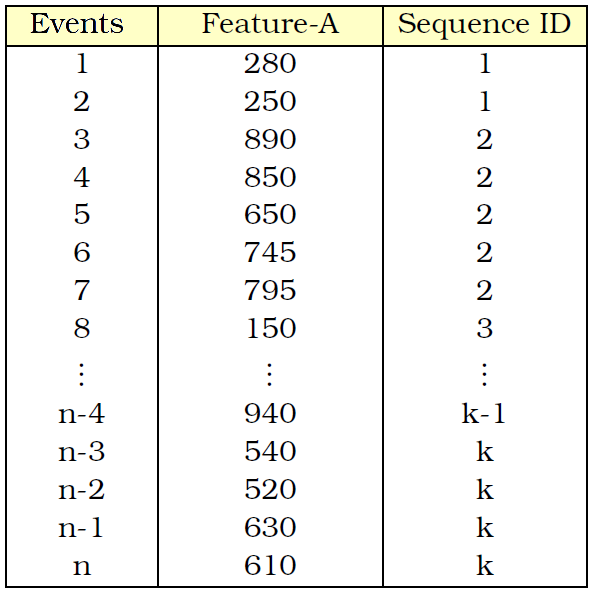
\includegraphics[height=4.5cm]{../tables/arbitrary_production_data_set.png}
		\[Lift(A\leftrightarrow B)=\frac{P(A,B)}{P(A)*P(B)}\]
		\column{.6\textwidth}
	\end{columns}
\end{frame}
\begin{frame}
	\frametitle{Association Networks}
	\begin{columns}[c]
		\column{.5\textwidth}
		\centering
		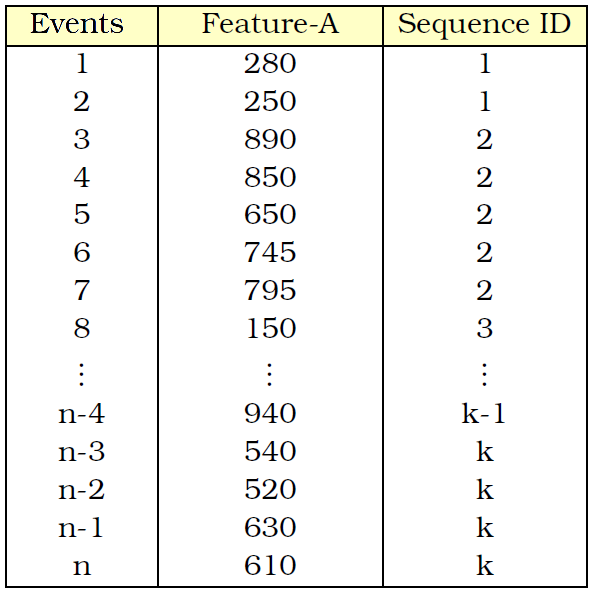
\includegraphics[height=4.5cm]{../tables/arbitrary_production_data_set.png}
		\[Lift(A\leftrightarrow B)=\frac{P(A,B)}{P(A)*P(B)}\]
		\column{.6\textwidth}
		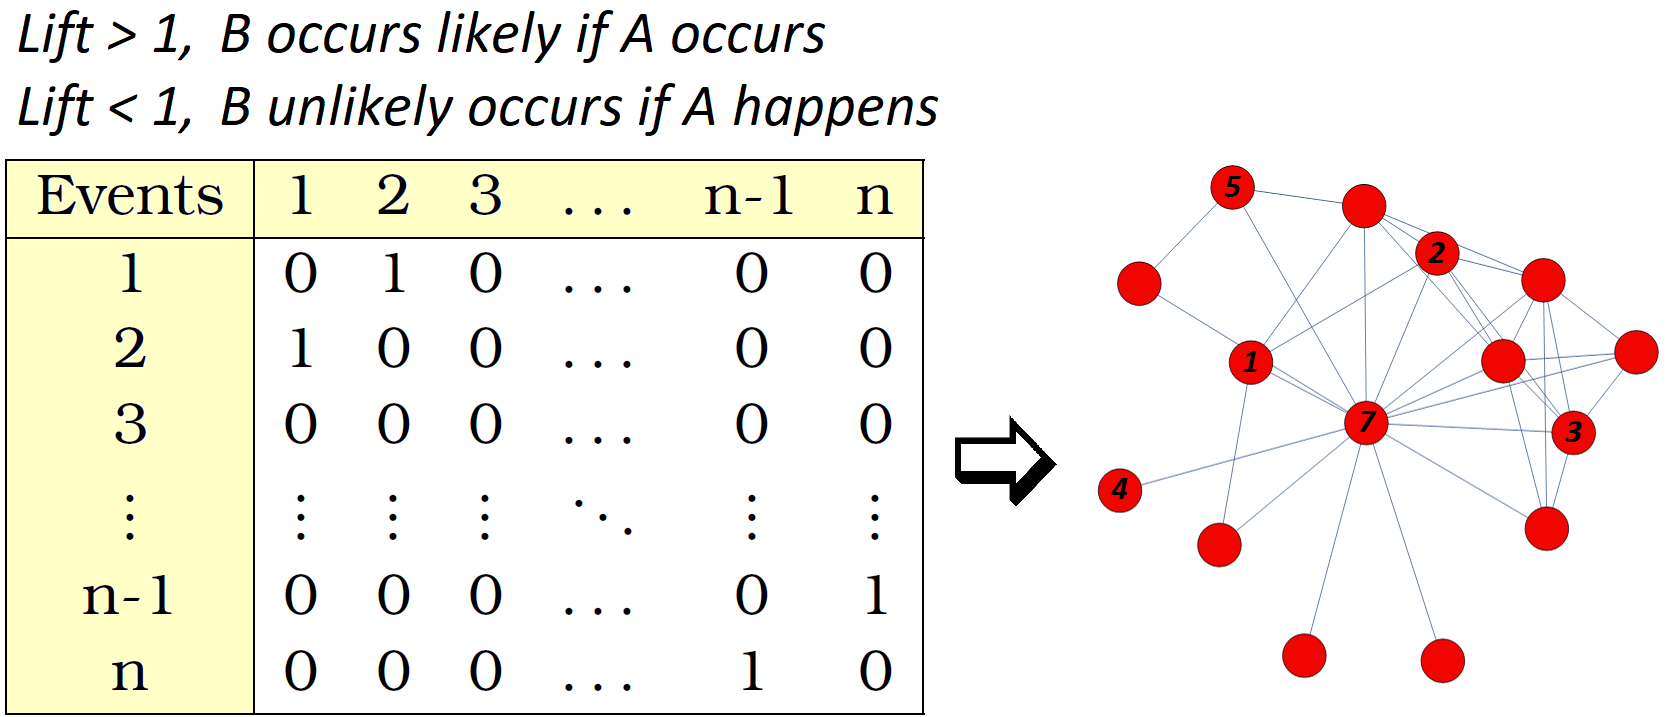
\includegraphics[width=8.5cm]{../tables/methodology-association-networks-adjacency_graph.png}
	\end{columns}
\end{frame}
%\subsubsection[Binning Schemes]{Binning Schemes}
\begin{frame}
	\frametitle{Binning Schemes}
	%\centering
	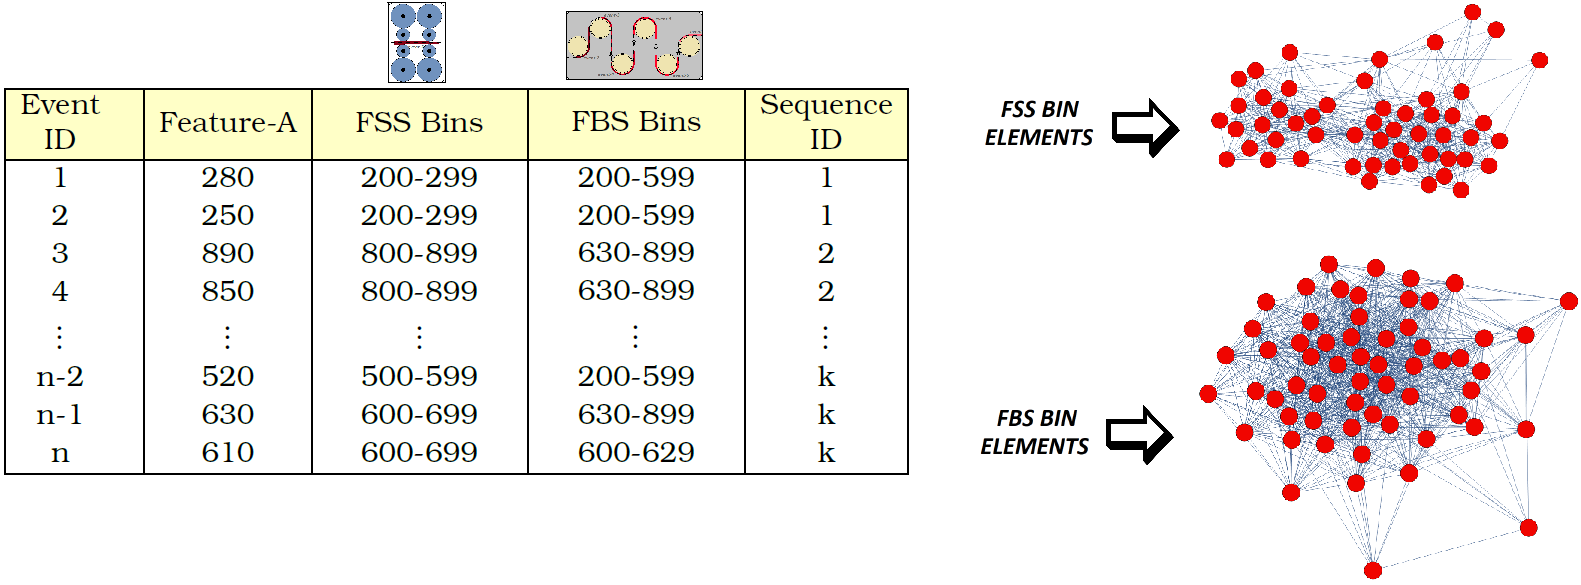
\includegraphics[width=\textwidth]{../tables/binning_schemes.png}
\end{frame}
%\subsubsection[Network Metrics Analysis]{Network Metrics Analysis}
\begin{frame}
	\frametitle{Network Metrics Analysis}
	\begin{columns}[c]
		\column{.55\textwidth}
		Modularity calculation was performed for the real network based on Newman (2006) formulated in his article.
		%\[Q = \frac {1} {4 m}\sum_ {ij} (A_{ij} - \frac {k_{i} k_{j}}{2 m}) s_{i} s_{j}\]
		\vspace{4cm}
		\column{.5\textwidth}
	\end{columns}
\end{frame}
\begin{frame}
	\frametitle{Network Metrics Analysis}
	\begin{columns}[c]
		\column{.55\textwidth}
		Modularity calculation was performed for the real network based on Newman (2006) formulated in his article.
		%\[Q = \frac {1} {4 m}\sum_ {ij} (A_{ij} - \frac {k_{i} k_{j}}{2 m}) s_{i} s_{j}\]
		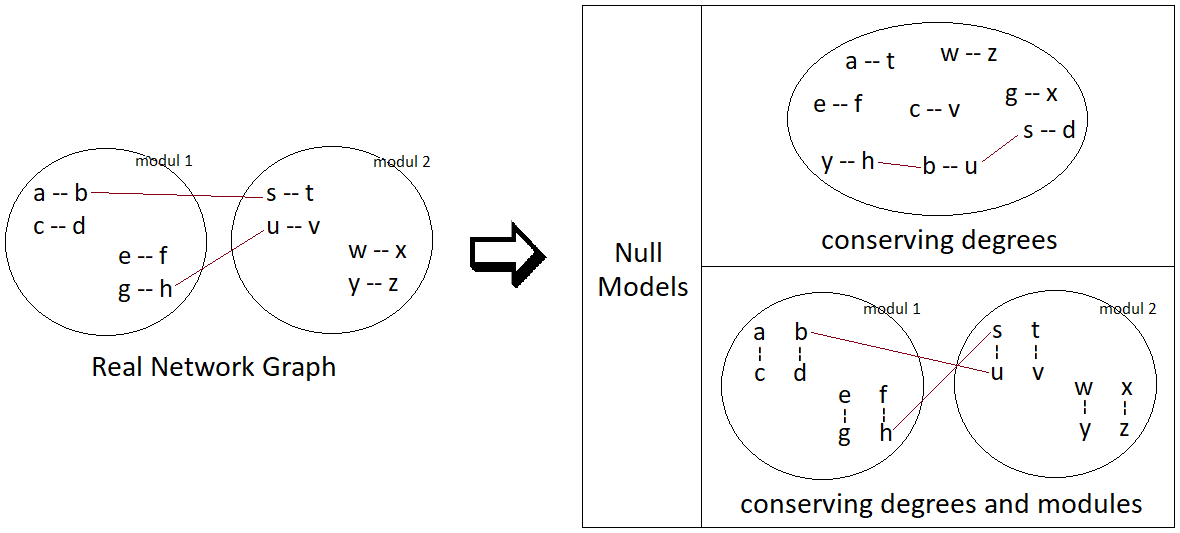
\includegraphics[width=\linewidth]{../tables/cartoon-null-model-definitions.png}
		\column{.5\textwidth}
	\end{columns}
\end{frame}
\begin{frame}
	\frametitle{Network Metrics Analysis}
	\begin{columns}[c]
		\column{.55\textwidth}
		Modularity calculation was performed for the real network based on Newman (2006) formulated in his article.
		%\[Q = \frac {1} {4 m}\sum_ {ij} (A_{ij} - \frac {k_{i} k_{j}}{2 m}) s_{i} s_{j}\]
		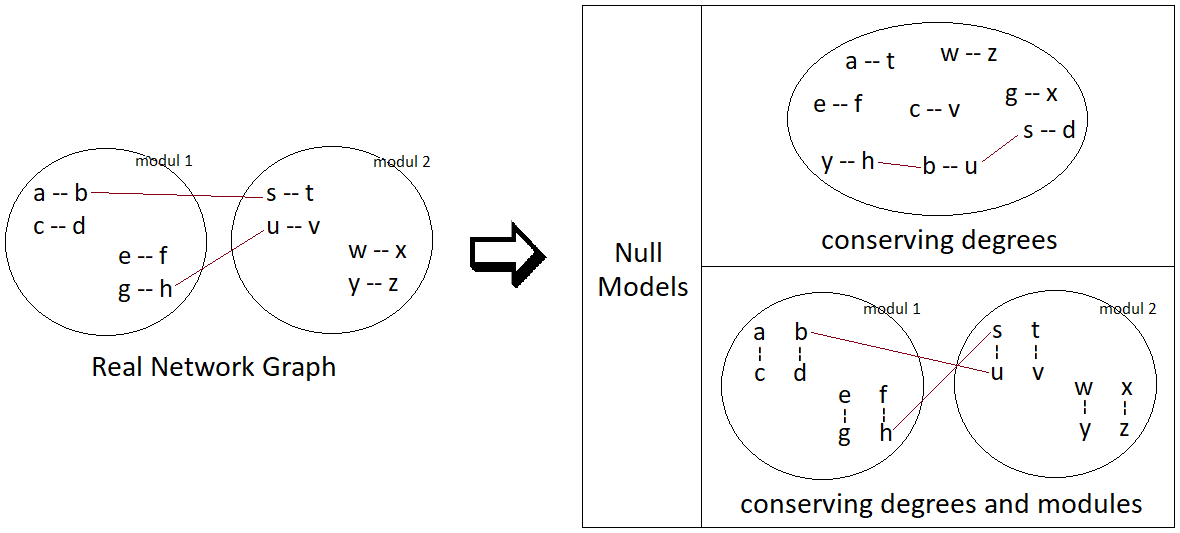
\includegraphics[width=\linewidth]{../tables/cartoon-null-model-definitions.png}
		\column{.5\textwidth}
		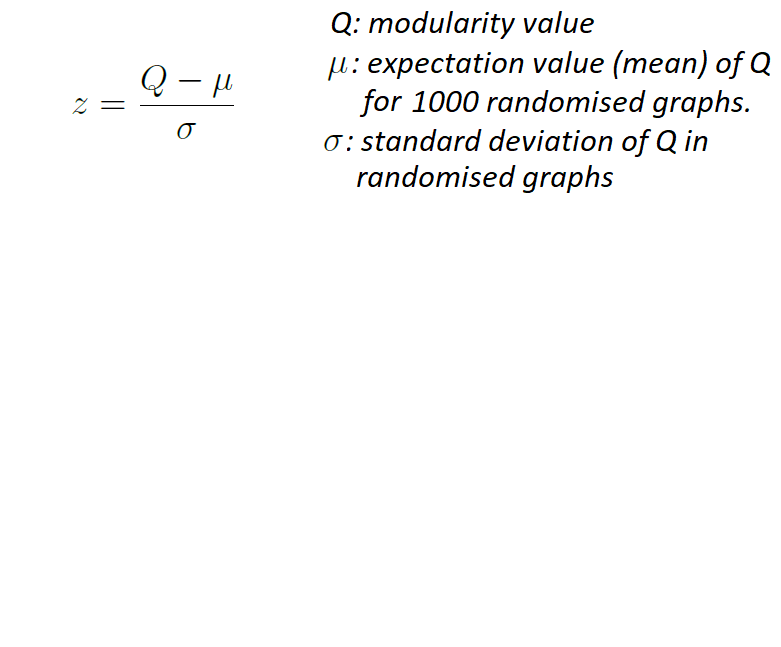
\includegraphics[width=\textwidth]{../tables/expected_network_structures_1.png}
	\end{columns}
\end{frame}
\begin{frame}
	\frametitle{Network Metrics Analysis}
	\begin{columns}[c]
		\column{.55\textwidth}
		Modularity calculation was performed for the real network based on Newman (2006) formulated in his article.
		%\[Q = \frac {1} {4 m}\sum_ {ij} (A_{ij} - \frac {k_{i} k_{j}}{2 m}) s_{i} s_{j}\]
		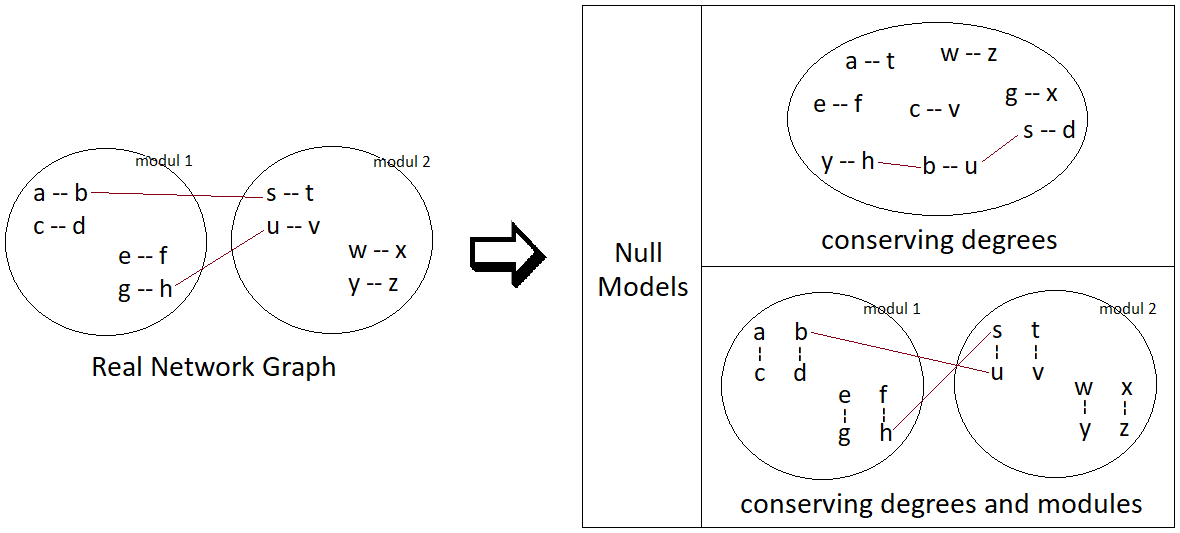
\includegraphics[width=\linewidth]{../tables/cartoon-null-model-definitions.png}
		\column{.5\textwidth}
		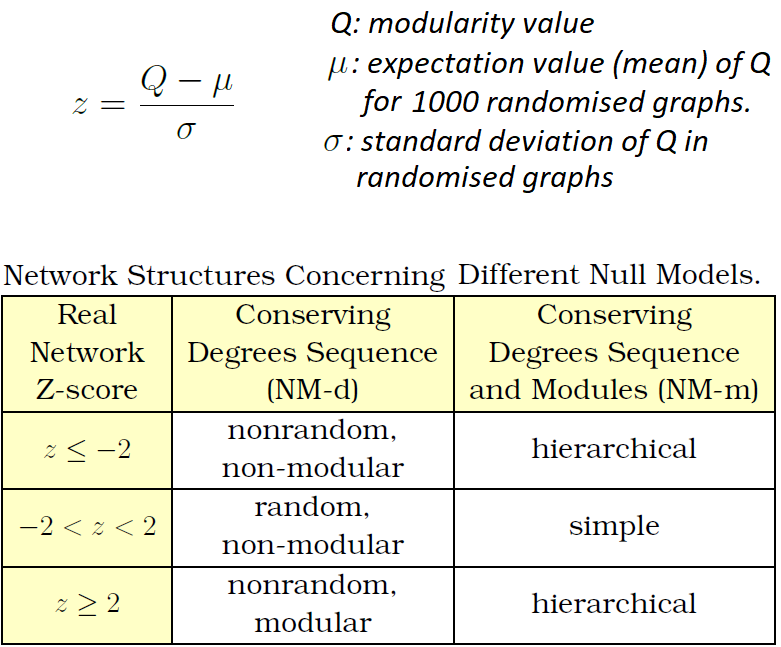
\includegraphics[width=\textwidth]{../tables/expected_network_structures_2.png}
	\end{columns}
\end{frame}